% Chapter 3
\chapter{Method and Implementation}
\label{chap:Chapter3}

This chapter details the methodology employed to tackle the problem, providing an overview of the technologies utilized and the implementation process. 

It consists of two sections: the first describes the method's design and proposed solutions, while the second covers the proof of concept, including implementation and optimization in a live environment.

\section{Method}
This section describes the methodological foundation of the project. 

It begins by presenting the technologies used and continues with an outline of three distinct solution strategies to the problem. 

Each approach is described through its pipeline and architectural design, offering a comparative view of possible solutions.

\subsection{Technological Overview}

The solution will be developed and implemented using the Python programming language, version 3.10.12. 
The following libraries are expected to be used throughout the development of the project:

\begin{itemize}
    \item \textbf{scikit-learn} (version 1.6.1): Machine learning models, including the Random Forest model and other necessary machine learning functionalities.
    \item \textbf{pandas} (version 2.2.3): Data manipulation and analysis, particularly for handling and processing alert datasets.
    \item \textbf{fastapi} (version 0.115.11): Building API, which will be used to expose endpoints for the system.
    \item \textbf{matplotlib} (version 3.10.1): Generating plots and graphs, particularly for data exploration or model evaluation.
    \item \textbf{SentenceTransformer} (likely needed): Text vectorization, particularly for converting text data into numerical embeddings.
\end{itemize}

\subsection{Problem-Solving Approaches}
This subsection analyzes three distinct approaches to tackling the identified problem. 
It outlines the specific methodologies employed for each approach, detailing the pipeline process involved and the architectural framework that supports its implementation.

\subsubsection{Random Forest with Reinforcement Learning Feedback Loop}

The first solution proposed in this study is a two-layered machine learning system that integrates a Random Forest model with a Reinforcement Learning feedback loop. 

This solution addresses the problem using a pre-trained RF model on historical data combined with an RL model that refines predictions based on analyst feedback.

\paragraph{Design} 

The RF model serves as the decision-making core, trained on a historical dataset of security alerts to classify incoming alerts by taxonomy and priority—\hyperref[objective3]{Objective 3}.

While the RF model provides strong initial predictions, it struggles to adapt to new attack vectors not represented in its training data. 
To address this, the RL model enhances the predictions made by the RF model and evaluates alerts as false positives or true positives, using feedback from security analysts.

Key features of this solution include:

\begin{itemize}
    \item The RL model adjusts its parameters through a continuous feedback loop, improving classification and generating confidence scores.
    \item This dynamic learning process ensures the system evolves with the ever-changing cybersecurity landscape.
    \item The system's adaptability helps manage false positives by learning patterns of false positives or true positives, refining its algorithms, and potentially reducing analysts' workloads.
    \item Designed to efficiently manage and analyze real-time alerts generated from a diverse range of log sources—\hyperref[objective4]{Objective 4}.
\end{itemize}

Integrating with IBM SOAR is vital for enhancing the overall effectiveness of the solution—\hyperref[objective5]{Objective 5}. 

IBM SOAR provides customization of dashboards presented to analysts, enabling:

\begin{itemize}
    \item Creation of custom fields where analysts can view the solution's outputs and mark them as correct or incorrect.
    \item Feedback from analysts, which is crucial for the RL model to learn from mistakes and improve over time.
\end{itemize}

This feedback loop supports continuous refinement and enhances accuracy for future predictions. 
Overall, this strategy leverages the strengths of supervised and reinforcement learning to create a robust solution for security alert triage. 
It enhances operational efficiency and threat response capabilities by:

\begin{itemize}
    \item Minimizing false positives through continuous improvement.
    \item Allowing integration with IBM SOAR to evaluate and test the solution's effectiveness in categorizing alerts and minimizing false positives—\hyperref[objective6]{Objective 6}.
\end{itemize}

\begin{figure}[h]
    \centering
    
\includegraphics[width=\textwidth]{ch3/assets/solution1_pipeline.png}
    \caption{Pipeline of the Random Forest with Reinforcement Learning Feedback Loop Solution}
    \label{fig:solution1_pipeline}
\end{figure}

\paragraph{Pipeline}

Figure~\ref{fig:solution1_pipeline} represents the data processing pipeline for this solution, which includes several key stages:

\begin{itemize}
    \item Raw security alert data is ingested and preprocessed for cleaning and feature extraction.
    \item A pre-trained RF model generates initial predictions on alert taxonomy and priority.
    \item A RL model refines these predictions using analyst feedback.
    \item The IBM SOAR analyst dashboard displays final predictions, including taxonomy, priority, false positive status, and confidence level.
    \item Analyst feedback is looped back to the RL model to improve classification accuracy over time.
\end{itemize}

\begin{figure}[h!]
    \centering
    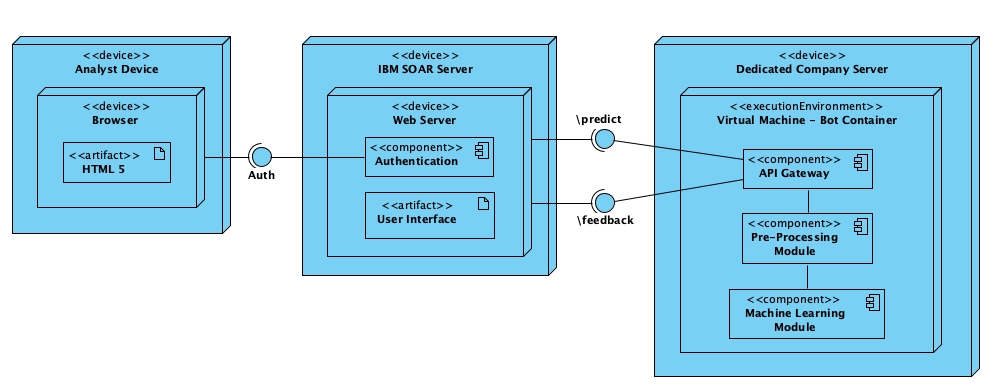
\includegraphics[width=\textwidth]{ch3/assets/Soltution1_Archquiteture.png}
    \caption{Architecture of the Random Forest with Reinforcement Learning Feedback Loop Solution}
    \label{fig:solution1_architecture}
\end{figure}

\paragraph{Architecture}

The diagram in Figure~\ref{fig:solution1_architecture} illustrates the architecture. It's organized into three major sections:

\begin{enumerate}
    \item \textbf{Analyst Device}: This device acts as the point of interaction where security analysts review and manage alerts. Represents the user interface. The analyst logs into the system through the \textbf{Authentication} component, enabling access to the dashboard.
    
    \item \textbf{IBM SOAR Server}: The IBM SOAR Server is the central system for managing security alerts. The server sends requests to the \textbf{Bot Container} through the \texttt{/predict} endpoint, triggering the alert classification process. Once the alert is processed, the \texttt{/feedback} endpoint is used to receive the analyst's input for further training of the RL model.
    
    \item \textbf{Dedicated Company Server}: The \textbf{Dedicated Company Server} hosts the \textbf{Bot Container}, which is deployed on a \textbf{Virtual Machine (VM)}. This container is responsible for the core functionality of the solution, consisting of three main components:
    \begin{itemize}
        \item \textbf{API Gateway}: This component serves as the entry point for receiving requests from the IBM SOAR Server and handling communication between the components inside the bot container. It processes the incoming alert data and forwards it to the appropriate modules.
        \item \textbf{Pre-Processing Module}: This module cleans and prepares the incoming alert data, extracting features and transforming them into a suitable format for the model.
        \item \textbf{Machine Learning Module}: The \textbf{Machine Learning Module} applies the \gls{RF} model to classify the alert. These predictions are then further refined through the \gls{RL} model.
    \end{itemize}
\end{enumerate}

This architecture is designed to be modular and scalable, allowing for easy integration with existing systems and the ability to adapt to evolving security threats.

\subsubsection{End-to-End Deep Learning Classifier with Feature Fusion}
A single \gls{DNN} trained end-to-end on labeled security alert data. 
It ingests enriched alert features that include raw SIEM logs, analyst comments, and metadata, using attention-based layers to identify the most relevant features. 
This model is deployed directly to make predictions and confidence scores in real time.

\textbf{Notes for later:}
\begin{itemize}
    \item \textbf{Objective 2:} Uses a \gls{DLM} that differs from classical \gls{ML}, designed to learn feature importance and complex relationships natively.
    \item \textbf{Objective 3:} Requires a well-labeled and feature-rich dataset, including alert content, origin, severity, and manual annotations.
    \item \textbf{Objective 4:} Connected to \gls{SIEM} for live alert feed; the model automatically classifies alerts in real time.
    \item \textbf{Objective 5:} Feedback can be sent to a retraining queue and influence future epochs (though less immediate than \gls{RL}).
    \item \textbf{Objective 6:} Evaluated based on prediction accuracy and feature attention relevance; may suffer from cold start and data scarcity issues.
\end{itemize}

\paragraph{Pipeline}
\paragraph{Architecture}

\subsubsection{Rule-Augmented Decision Tree with Feedback Aggregation}
A hybrid system combining static expert rules with a lightweight \gls{DTC}. 
The rule engine pre-filters known benign or critical alert patterns before passing unknown or ambiguous cases to a \gls{DTM}. 
Feedback is logged and reviewed in batch to update the rule base and retrain the decision tree periodically.

\textbf{Notes for later:}
\begin{itemize}
    \item \textbf{Objective 2:} Incorporates domain knowledge (rules) with a basic \gls{ML} model, reducing complexity while offering interpretability.
    \item \textbf{Objective 3:} Relies on a clean and segmented dataset to distinguish known from unknown patterns.
    \item \textbf{Objective 4:} Integrated with \gls{SIEM} for real-time alert tagging and rule matching before \gls{ML} classification.
    \item \textbf{Objective 5:} Feedback is collected but applied asynchronously (e.g., weekly retraining and rule review).
    \item \textbf{Objective 6:} Effective for low-volume environments; easily auditable but less dynamic in response to new threats.
\end{itemize}

\paragraph{Pipeline}
\paragraph{Architecture}

%----------------------------------------------------------------------------------------

\subsection{Comparative Analysis}
This subsection presents a comparison of the three proposed approaches based on key evaluation criteria. 
The goal is to assess their suitability in the context of a real-world SOC environment, taking into consideration implementation complexity, adaptability, performance, interpretability, and integration potential.

\captionsetup[table]{font=small} % Set the caption font size
\scriptsize % Reduce the font size for the table content
\begin{longtable}{@{}P{3cm}P{3cm}P{4cm}P{4cm}@{}}
    \caption{Comparison of Proposed Solutions}
    \label{tab:solution_comparison} \\
    \toprule
    \textbf{Criteria} & \textbf{\gls{RF} + \gls{RL}} & \textbf{\gls{DNN}} & \textbf{Rules + Decision Tree} \\
    \midrule
    \endfirsthead

    \toprule
    \textbf{Criteria} & \textbf{\gls{RF} + \gls{RL}} & \textbf{\gls{DNN}} & \textbf{Rules + Decision Tree} \\
    \midrule
    \endhead

    \bottomrule
    \endfoot

    \bottomrule
    \endlastfoot

    Architecture Type & \gls{RF} + \gls{RL} (Two-layer) & \gls{DNN} & Rule-based + Decision Tree \\
    \vspace{0.2cm}
    Implementation Complexity & Moderate & High & Low \\
    \vspace{0.2cm}
    Adaptability to New Threats & High (via \gls{RL}) & Moderate (via retraining) & Low (manual updates) \\
    \vspace{0.2cm}
    Learning from Feedback & Online (via \gls{RL}) & Periodic retraining & Batch/manual integration \\
    \vspace{0.2cm}
    Cold Start Handling & Excellent (\gls{RF} pre-trained) & Poor & Excellent (rules pre-set) \\
    \vspace{0.2cm}
    Interpretability & Moderate & Low & High \\
    \vspace{0.2cm}
    Scalability & High & High & Moderate \\
    \vspace{0.2cm}
    Integration with SIEM (IBM SOAR) & Easy & Easy & Easy \\
    \vspace{0.2cm}
    False Positive Reduction & Adaptive (confidence scoring) & Model confidence only & Rigid (rule-defined) \\
    \vspace{0.2cm}
    Performance in Evolving Scenarios & High & Moderate & Low \\
    
\end{longtable}

\normalsize

\textbf{Notes for Analysis:}
\begin{itemize}
    \item \textbf{Solution 1} stands out by combining the stability and maturity of \gls{RF} with the adaptability and feedback-driven refinement of \gls{RL}.
    \item Its \textit{cold start} advantage means it can be deployed immediately, using \gls{RF} predictions while the \gls{RL} model adapts gradually.
    \item It offers a built-in mechanism for minimizing false positives via the \gls{RL} layer, which adjusts the \gls{RF} output and adds a confidence score.
    \item Although Solution 2 is theoretically powerful, it requires extensive data, compute, and time to reach maturity—posing risks in production environments.
    \item Solution 3 is simple and interpretable but lacks the adaptability and intelligence needed for dynamic cybersecurity environments, relying too heavily on static rules.
    \item Considering the requirements of real-time alert classification, feedback learning, and SOC integration, Solution 1 offers the best balance of robustness, scalability, and long-term adaptability.
\end{itemize}


\section{Proof of Concept}
This section presents the practical implementation of the proposed solution, including the setup of the test environment, preparation of the dataset, and execution of the machine learning models. It aims to demonstrate the feasibility and performance of the selected approach under realistic conditions.

\subsection{Dataset Division}
This subsection details how the dataset was split for training, validation, and testing.

\subsection{Data Processing}
Explanation of how the raw data was prepared for use in the machine learning pipeline.

\subsection{Data Normalization}
Discussion of normalization techniques applied to the data to improve model performance.

\subsection{Machine Learning Model Development}
In this section, the implementation of selected machine learning algorithms is discussed.

\subsection{Hyperparameter Tuning}
Details of the strategy used to tune hyperparameters and optimize the models' performance.
